\documentclass{article}
\usepackage[section]{placeins}
\usepackage{graphicx}
\usepackage{wrapfig}

\usepackage{hyperref}
\hypersetup{
    colorlinks=true,
    linkcolor=blue,
    filecolor=magenta,      
    urlcolor=cyan,
    pdftitle={Overleaf Example},
    pdfpagemode=FullScreen,
    }

\author{Yaghoub Shahmari}
\title{Report - Problem Set no 4}
\date{\today}
\graphicspath{ {../Figs/} }

\begin{document}
    \maketitle
    \section*{Problem 1}
    \textbf{Basic description:}
    In this problem, we try to find the chance of being connected to the infinite cluster again.
    The difference from the previous attempt is that I use the fraction of the size of the infinite
    cluster to the size of the whole network. So all of the previous steps will go through.

    \textbf{Results:}

    \begin{figure}[!htb]
        \centering
        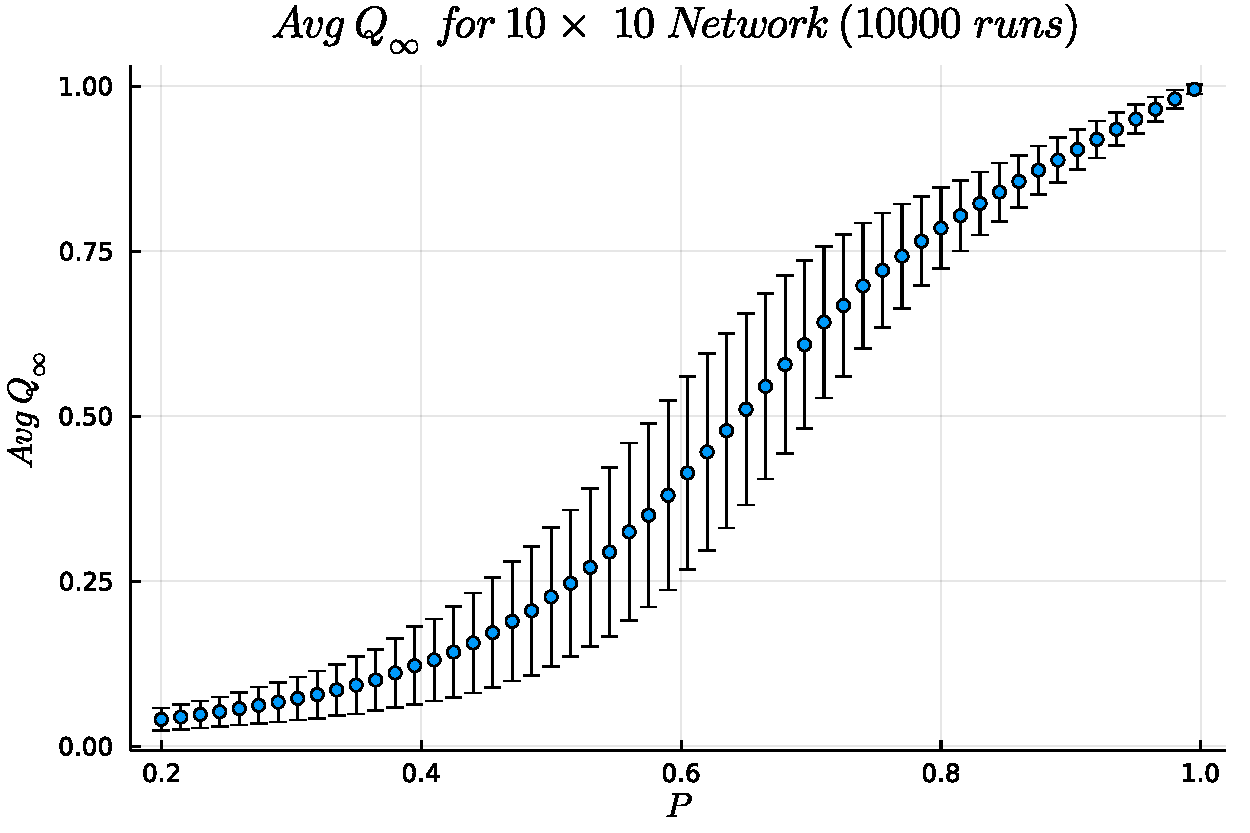
\includegraphics[scale = 0.275]{/Q1/dim10-10000}
        \label{fig:1.1}
        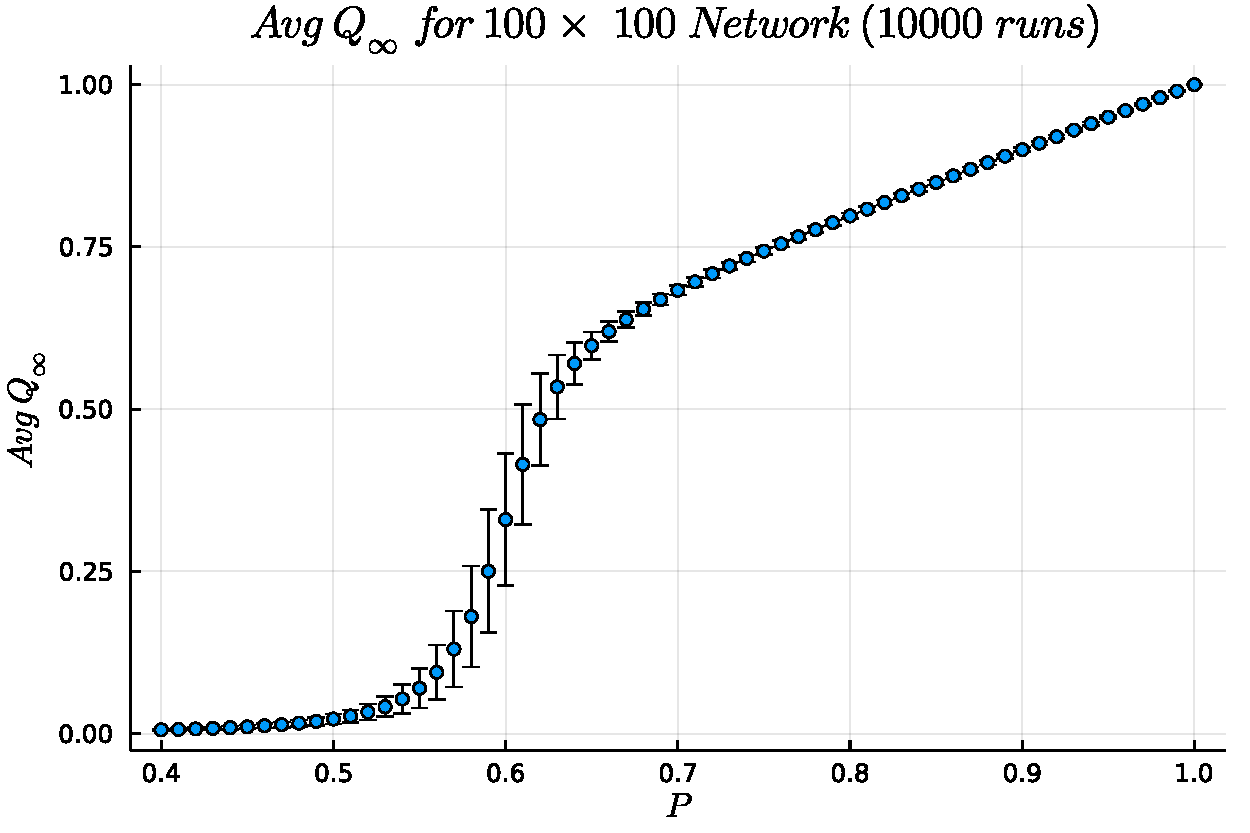
\includegraphics[scale = 0.275]{/Q1/dim100-10000}
        \label{fig:1.2}
        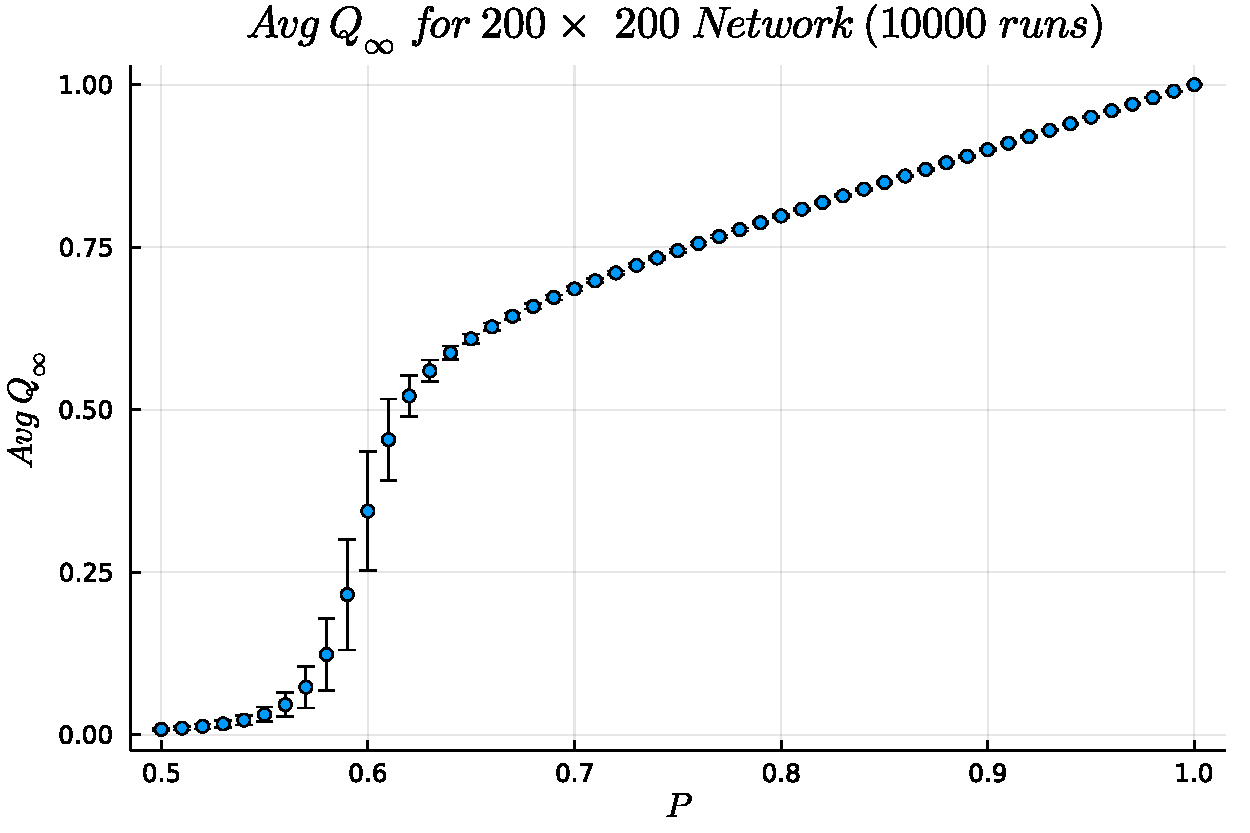
\includegraphics[scale = 0.4]{/Q1/dim200-10000}
        \label{fig:1.3}
        \caption{$Q_{\infty}$ for $L=10, 100, 200$}
    \end{figure}

    \pagebreak

    \section*{Problem 2}
    \textbf{Basic description:}

    In this problem, we try to find the correlation length of percolation of grid graphs.
    In this case, we will find the largest finite cluster.
    Then, we have to calculate the gyration radius of that cluster as the book told us.
    and finally, we will run the calculation and average the data.

    \textbf{Results:}

    \begin{figure}[!htb]
        \centering
        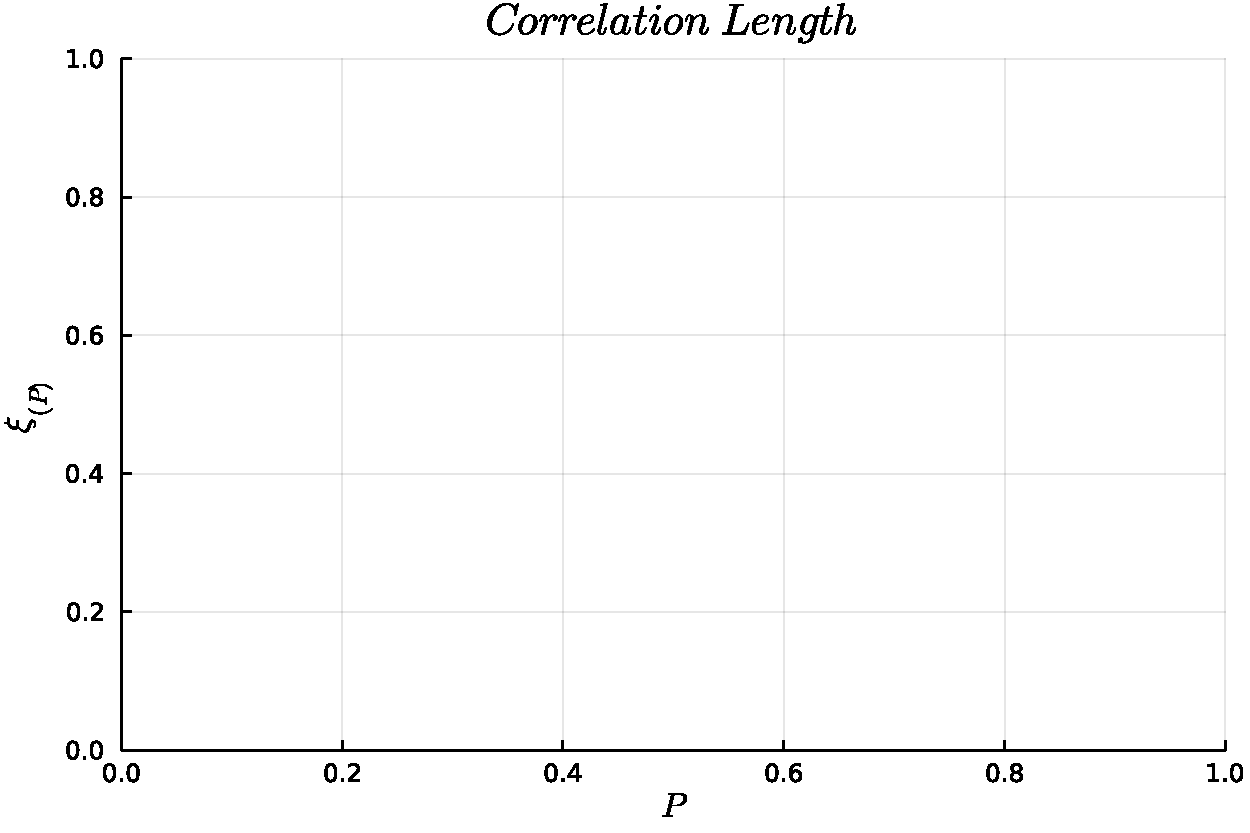
\includegraphics[scale = 0.2]{/Q2/CL}
        \label{fig:2.1}
        \caption{$Q_{\infty}$ for $L=10, 100, 200$}
    \end{figure}

    \textbf{Extrapolation results:}

    To find the requested parameters ($\nu$ and $Pc_{\infty}$),
    we have to do previous steps for several $P$ and $L$.
    After exporting data, we use the Curvefit function in the LsqFit library.
    Given that we intend to find the parameters and improve the
    accuracy we will consider that we know one of the parameters (find the amount from the internet)
    and find the other using the mentioned method.

    \begin{figure}[!htb]
        \centering
        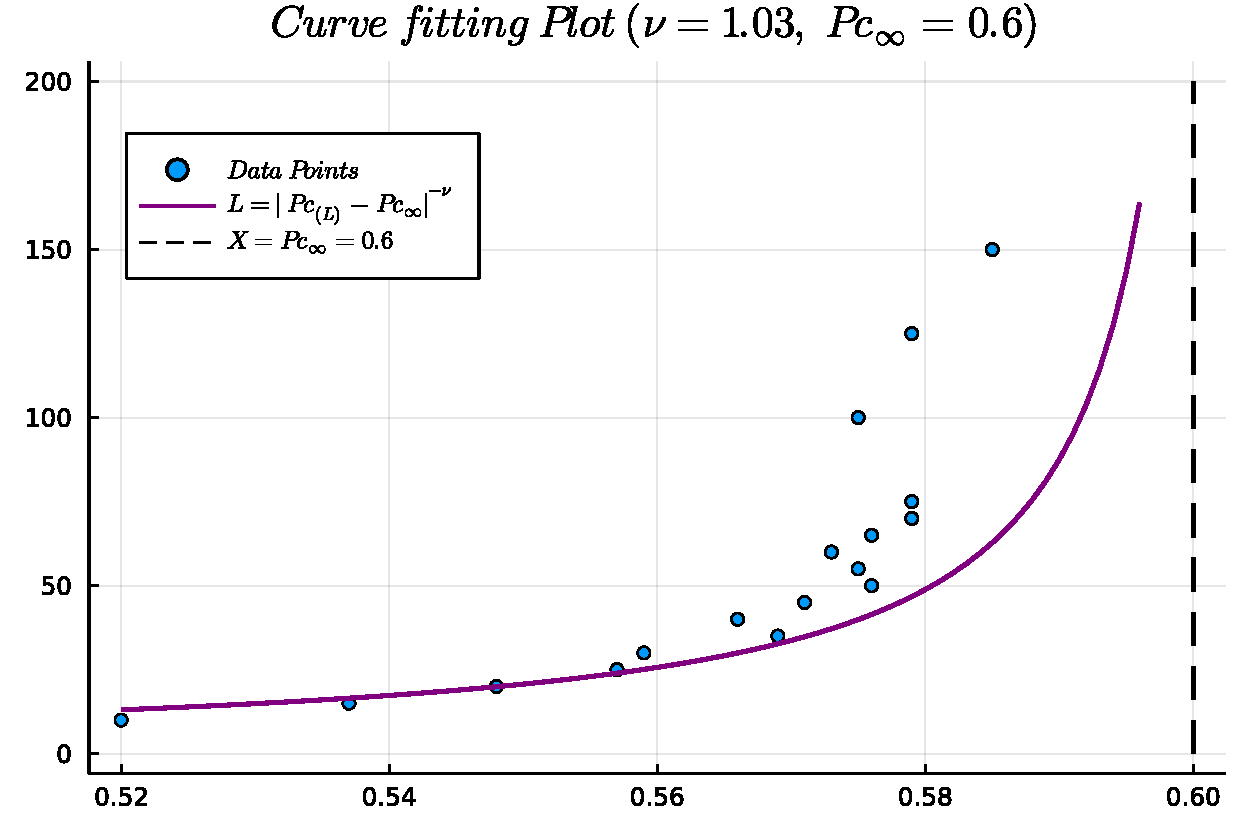
\includegraphics[scale = 0.35]{/Q2/Q2-CF-res}
        \label{fig:2.2}
        \caption{Curvefit result for exported data}
    \end{figure}
    
\end{document}